

\documentclass[11pt]{article}

\usepackage{amsmath}
\usepackage[pdftex]{graphicx}
\usepackage{color}
\usepackage{hyperref}   %Aktive internett referanser. Medfører også aktive referanes til figurer
\usepackage{float}  
\usepackage{listings} 

\newcommand{\beq}{\begin{equation}}
\newcommand{\eeq}{\end{equation}}
\newcommand{\beqa}{\begin{eqnarray}}
\newcommand{\eeqa}{\end{eqnarray}}  

\title{\bf FYS4150, Computational Physics \\Project 1}

\author{Andreas Bjurstedt}

\date{\today}
% Hint: \title{what ever}, \author{who care} and \date{when ever} could stand 
% before or after the \begin{document} command 
% BUT the \maketitle command MUST come AFTER the \begin{document} command! 
\begin{document}

\maketitle


%\begin{abstract}
%Short introduction to subject of the paper \ldots 
%\end{abstract}

\subsection*{Abstract}
The one-dimensional Poisson equation with Dirichlet boundary conditions is solved numerically
by rewriting it as a set of linear equations. In the matrix form 
$\mathbf{Av} = \mathbf d$ of the linear equation set, the quadratic matrix $\mathbf A$
is tridiagonal. Three algoritms for solving the linear equation set and find
the discrete, approximate solution ${\mathbf v}$ are presented and tested. Two of them are
more time efficient than the third one. They calculate an aproximate solution which
converge towards the given analytical solution as the number of gridpoints $n$ increases up
towards $n = 10^7$. Then the accumulation of round off errors due to loss of significant bits
leads to less accurate approximate solutions again. The third algoritm are more generalized
and less time efficient than the other two. It also need all the zero elements in $\mathbf A$
in order to function. This lead to problems with lack of internal computer memory as the number 
of grid points $n$ increases towards $n=10^5$. 

\subsection*{Introduction}
In this project we solve the one-dimentional Poisson equation with Dirichlet 
boundary conditions numerically and compare the numerical solution we find with a given 
analytical solution of the equation. Taylor expansion of the general solution $u(x)$ leads to
an approximate expression of its second derivative $u''(x)$ on the equation's left hand side.
The equation can then be rewritten as a set on $n$ linear equations with $n$ unknowns, where
$n$ is the number of gridpoints in the solution of the linear equation set. The solution of
the equation set is the discrete, approximate solution to the Poisson equation. In the matrix form 
$\mathbf{Av} = \mathbf d$ of the linear equation set, the quadratic matrix $\mathbf A$
is tridiagonal. The element value on the matrix diagonal is 
$b_{ii} = 2, \hspace{4mm} i = 1, \cdots, n$
Just below and above the diagonal, the element value is -1:
$a_{i+1,i} = -1, \hspace{4mm} i = 1, \cdots, n-1$ and $c_{i,i+1} = -1, 
\hspace{4mm} i = 1, \cdots, n -1$.
The value of the rest of the matrix elements are equal to zero.

\vspace{4mm}
\noindent
The first algorithm we present to find the numerical solution exploit the triagonal property 
of the matrix. It doens't require that all the matrix elements on a diagonal has the same
value. As input it need three vectors, $\mathbf a$ $\mathbf b$ and $\mathbf c$ to represent
the matrix $\mathbf A$.

\vspace{4mm}
\noindent
The second algorithm we present in addition also exploit the fact that all the elements on a diagonal
has the same value. As input it only need three constants, $a$ $b$ and $ c$ to represent
the matrix $\mathbf A$. This is the most efficient algorithm in our special case.

\vspace{4mm}
\noindent
The third algorithm is based on LU decomposition of the matrix and can solve any linear set of
n equation with n unknowns, as long as the matrix $\mathbf A$ is invertible. As input it
needs the complete matrix with all the zero elements. This is not an efficient algorithm in
our special case.

\vspace{4mm}
\noindent
The algorithms are tested in terms of how well they converge towards the analytical solution
for an increasing number of grid points $n$ and how time efficient they are. The results
are presented in the \textbf{Results} section. 


\subsection*{Methods}
The one-dimensional Poisson equation with Dirichlet boundary conditions is given as:

\begin{equation}
-u''(x) = f(x), \hspace{0.5cm} x\in(0,1), \hspace{0.5cm} u(0) = u(1) = 0
\label{lig1}
\end{equation}
In this project we will assume that $f(x) = 100e^{-10x}$. Then the analytical solution in 
closed form is not difficult to find. Just integrate twice and use the boundary conditions 
to decide the two integration constants. The result is

\begin{equation*}
u(x) = 1-(1-e^{-10})x-e^{-10x}
\label{lig2}
\end{equation*}
The analytical solution is useful when we evaluate the numerical method, where we apply
an approximation to the second derivative $u''(x)$. The numerical method and the
associated computer algorithms described here, can be found in \cite{mhh}. 
A Taylor expansion of $u(x)$  gives

\begin{equation*}
u(x + h) = u(x) + hu'(x) + h^2\frac{u''(x)}{2!} + h^3\frac{u^{(3)}(x)}{3!} 
+ h^4\frac{u^{(4)}(x)}{4!} + \cdots
\end{equation*}
An alternative Taylor expansion is

\begin{equation*}
u(x - h) = u(x) - hu'(x) + h^2\frac{u''(x)}{2!} - h^3\frac{u^{(3)}(x)}{3!} 
+ h^4\frac{u^{(4)}(x)}{4!} - \cdots
\end{equation*}
Combining them, we get

\begin{equation*}
u(x+h) +u(x-h) = 2u(x) + 2h^2\frac{u''(x)}{2!} +2h^4\frac{u^{(4)}(x)}{4!} + \cdots
\end{equation*}
and

\begin{equation*}
u''(x) = \frac{u(x+h)-2u(x)+u(x-h)}{h^2}-2h^2\frac{u^{(4)}(x)}{4!}-2h^4\frac{u^{(6)}(x)}{6!}
- \cdots 
\end{equation*}
which with $O(h^2)$ notation becomes

\begin{equation*}
u''(x) = \frac{u(x+h)-2u(x)+u(x-h)}{h^2} + O(h^2)
\end{equation*}
For small $h$, we can omit the $O(h^2)$ term. Replacing $u''(x)$ with this approximation, we 
now have an aproximation of expression (\ref{lig1}) which form a basis for a discrete 
approximation and the numerical algorithms we will apply.
\begin{equation}
-\frac{u(x+h)-2u(x)+u(x-h)}{h^2} = f(x), \hspace{0.3cm} x\in(0,1), \hspace{0.3cm} u(0) = u(1) = 0
\label{lig2}
\end{equation}
In a discrete approximation we have discrete points. We apply $n+2$ discrete points, where the
distance between them is
\begin{equation*}
h = \frac{1}{n+1}
\end{equation*}
and 
\begin{equation*}
x_i = ih,  \hspace{0.3cm} i = 1, 2, \cdots, n
\end{equation*}
The discrete approximation of expression (\ref{lig1}) then becomes 
\begin{equation}
-v_{i-1}+2v_i-v_{i+1} = h^2f_i, \hspace{0.3cm} v_0 = v_{n+1} = 0
\label{lig3}
\end{equation}
As a simple illustration, let n = 4. Expression (\ref{lig3}) then gives

\begin{eqnarray*}
2v_1 - v_2 &=& h^2f_1  \hspace{0.5cm} (n = 1)\\
-v_1 + 2v_2 - v_3 &=&h^2f_2  \hspace{0.5cm} (n = 2)\\
-v_2 + 2v_3 - v_4 &=&h^2f_3  \hspace{0.5cm} (n = 3)\\
-v_3 + 2v_4  &=&h^2f_4  \hspace{0.5cm} (n = 4)\\
\end{eqnarray*} 
This is four linear equations with four unknowns, which on matrix form becomes

\[
\begin{bmatrix}
  2 & -2 & 0 & 0 \\
 -1 & 2 & -1 &  0 \\
  0 & -1 & 2 & -1 \\
  0 & 0 & -1 & 2\\   
\end{bmatrix}
\begin{bmatrix}
v_1\\v_2\\v_3\\v_4
\end{bmatrix}
= h^2
\begin{bmatrix}
f_1\\f_2\\f_3\\f_4
\end{bmatrix}
\]
A more compact notation of this matrix form is $\mathbf{A}\mathbf{v} = \tilde{\mathbf{d}}$. For
any $n>3$ we just get a generalization of what is explained above

\[
\begin{bmatrix}
    2& -1& 0 &\dots   & \dots &0 \\
    -1 & 2 & -1 &0 &\dots &\dots \\
     0&-1 &2 & -1 & 0 & \dots \\
     & \dots   & \dots &\dots   &\dots & \dots \\
     0&\dots   &  &-1 &2& -1 \\
     0&\dots    &  & 0  &-1 & 2 \\
\end{bmatrix}
\begin{bmatrix}
      v_1\\
      v_2\\
      \dots \\
      \dots  \\
      \dots \\
      v_n\\
\end{bmatrix}
=\begin{bmatrix}
      d_1\\
      d_2\\
      \dots \\
      \dots \\
      \dots \\
      d_n\\
\end{bmatrix}
\]
I order to solve this system of linear equations and find the discrete approximation $\mathbf{v}$ of
$u(x)$, we will look at three numerical algorithms. The two first ones exploits the fact that
the matrix $\mathbf{A}$ is tridiagonal.

\vspace{4mm}
\noindent
The first algorithm is able to solve the system with the tridiagonal matrix $\mathbf{A}$ on a general
form. We have 

\[
\begin{bmatrix}
    b_1 & c_1 & 0   &\dots & \dots & \dots \\
    a_2 & b_2 & c_2 & \dots& \dots & \dots \\
        & a_3 & b_3 & c_3  & \dots & \dots \\
        &\dots&\dots &\dots  &\dots & \dots \\
     & &  &a_{n-1}&b_{n-1} &c_{n-1} \\
     &    &  &  & a_{n} & b_n \\
\end{bmatrix}
\begin{bmatrix}
      v_1\\
      v_2\\
      \dots \\
      \dots  \\
      \dots \\
      v_n\\
\end{bmatrix}
=\begin{bmatrix}
      {d}_1\\
      {d}_2\\
      \dots \\
      \dots \\
      \dots \\
      {d}_n\\
\end{bmatrix}
\]
The first step is to solve this system is to get $\mathbf{A}$ on an upper triangular form,
witch means $a_2 = a_3 = \cdots = a_{n} = 0$. We achieve this by calculating

\begin{eqnarray*}
\tilde{b}_i &=& b_i -\frac{a_i}{\tilde{b}_{i-1}}c_{i-1}\\
\tilde{d}_i &=& d_i -\frac{a_i}{\tilde{b}_{i-1}}\tilde{d}_{i-1}
\hspace{0.3cm} \text{for} \hspace{0.3cm} i = 2, \cdots, n  
\end{eqnarray*}
We then get
\begin{equation*}
\tilde{a}_i = a_i -\frac{a_i}{\tilde{b}_{i-1}}\tilde{b}_{i-1} = 0
\end{equation*}
as we want. This step is called forvard substitution. For forward substitution, we see that
for each step $i$ we have
5 operartions (addition, subtraction, multiplication, division) between floating points, that
is 5 flops. 

\vspace{4mm}
\noindent
Our matrix system now look like this

\[
\begin{bmatrix}
    b_1 & c_1 & 0   &\dots & \dots & \dots \\
    0 & \tilde{b}_2 & c_2 & \dots& \dots & \dots \\
        & 0 & \tilde{b}_3 & c_3  & \dots & \dots \\
        &\dots&\dots &\dots  &\dots & \dots \\
     & &  &0 &\tilde{b}_{n-1} &c_{n-1} \\
     &    &  &  & 0 & \tilde{b}_n \\
\end{bmatrix}
\begin{bmatrix}
      v_1\\
      v_2\\
      \dots \\
      \dots  \\
      \dots \\
      v_n\\
\end{bmatrix}
=\begin{bmatrix}
      d_1\\
      \tilde{d}_2\\
      \dots \\
      \dots \\
      \dots \\
      \tilde{d}_n\\
\end{bmatrix}
\]
We can now find $v$ by starting with the last equation in the system. When we know $v_n$, we
can find $v_{n-1}$, when we know $v_{n-1}$ we can find $v_{n-2}$ and so on
    
\begin{equation*}
v_n = \frac{\tilde{d}_n}{\tilde{b}_n}
\end{equation*}
and
\begin{equation*}
v_{i-1} = \frac{\tilde{d}_{i-1}-c_{i-1}v_i}{\tilde{b}_{i-1}}
\hspace{0.3cm} \text{for} \hspace{0.3cm} i = n, n-1, \cdots, 2  
\end{equation*}
This step is called backward substitution. For backward substitution, we see that we have 3 flops 
for each step $i$, and in addittion one flop extra
for calculating $v_n$. In total $(5+3)(n-1) + 1 = 8(n-1) + 1$ flops are therefor needed for 
the algorithm (forward substitution and backward substitution) to
calculate its way through its $n-1$ steps and find $\mathbf{v}$ when the matrix $\mathbf{A}$ has a
general tridiagonal form.
For later references we call this algorithm 
\emph{The general tridiagonal algorithm} or simply \emph{algorithm 1}. As input we see
that it only need three vectors, $\mathbf a$ $\mathbf b$ and $\mathbf c$ to represent
the matrix $\mathbf A$.

\vspace{4mm}
\noindent
In the second algorithm we exploits the fact that actually
\begin{eqnarray*}
a_2 &=& a_3 = \cdots = a_i = \cdots = a_{n} = -1\\
b_1 &=& b_2 = \cdots = b_i = \cdots = b_{n} = 2\\
c_1 &=& c_2 = \cdots = c_i = \cdots = c_{n-1} = -1\\
\end{eqnarray*}
in the tridiagonal matrix $\mathbf{A}$. We can then simplify the expressions for $\tilde{b_i}$,
$\tilde{d_i}$ in the forward substitution step, and for $v_i$ in the backward substitution step
given above. In the forward substitution step we get 
\begin{eqnarray*}
\tilde{b}_2 &=& \frac{3}{2}\\
\tilde{d}_2 &=& d_2 + \frac{1}{2} d_1\\
\tilde{b}_3 &=& \frac{4}{3}\\
\tilde{d}_3 &=& d_3 + \frac{2}{3}\tilde{d}_2\\
\tilde{b}_4 &=& \frac{5}{4}\\
\tilde{d}_4 &=& d_4 + \frac{3}{4}\tilde{d}_3\\
\end{eqnarray*}
and so on. We see the pattern and get
\begin{eqnarray*}
\tilde{b}_i &=& \frac{i+1}{i}\\
\tilde{d}_i &=& d_i + \frac{i-1}{i}\tilde{d}_{i-1}
\hspace{0.5cm} \text{for} \hspace{0.3cm} i = 2, \cdots, n  
\end{eqnarray*}
in the forward substitution step. We see that now the number of flops in each forward
substitution step $i$ is reduced to 2. In a similar way, the backward substitution step is also
simplified. We get 

\begin{equation*}
v_n = \frac{\tilde{d}_n}{\tilde{b}_n}
\end{equation*}
and
\begin{equation*}
v_{i-1} = \frac{\tilde{d}_{i-1} + v_i}{\tilde{b}_{i-1}}\\
        = \frac{i-1}{i}(\tilde{d}_{i-1}+ v_i)
\hspace{0.5cm} \text{for} \hspace{0.3cm} i = n, n-1, \cdots, 2  
\end{equation*}
The number of flops in each backward substitution step $i$ is also reduced to 2, and in addition
we have one flop
extra for calculating $v_n$. In total $(2+2)(n-1) + 1 = 4(n-1) +1$ flops are therefor needed
for the algorithm to calculate its way through its $n-1$ steps and find $\mathbf v$ when the 
matrix $\mathbf{A}$ is simplified from its general tridiagonal form. 
For later references we call this algorithm 
\emph{The special tridiagonal algorithm} or simply \emph{algorithm 2}. As input we see
that it only needs three constants, $ a$ $b$ and $c$ to represent
the matrix $\mathbf A$.

\vspace{4mm}
\noindent
The third algorithm is the most general one. Here we omit the fact that the matrix $\mathbf{A}$
is tridiagonal, and assume that the matrix form of the set of linear equations is given as

\[
\begin{bmatrix}
    a_{11} & a_{12} & \dots   &\dots & \dots & a_{1n} \\
    a_{21} & a_{22} & \dots & \dots& \dots & a_{2n} \\
     a_{31} & a_{32} & \dots  & \dots & \dots & a_{3n} \\
    \dots &\dots&\dots &\dots  &\dots & \dots \\
     & &  & &a_{n-1, n-1} &a_{n-1,n} \\
     &    &  &  &  & a_{n,n} \\
\end{bmatrix}
\begin{bmatrix}
      v_1\\
      v_2\\
      \dots \\
      \dots  \\
      \dots \\
      v_n\\
\end{bmatrix}
=\begin{bmatrix}
      d_1\\
      d_2\\
      \dots \\
      \dots \\
      \dots \\
      d_n\\
\end{bmatrix}
\]
In order to find $\mathbf{v}$, we apply LU decomposition on the matrix $\mathbf{A}$ and exploit
that the lower triangular matrix $\mathbf{L}$ is invertible. Applying LU decoposition on
$\mathbf{A}$ we get

\begin{equation*}
\mathbf{Av} = \mathbf{LUv} = \mathbf{d}
\end{equation*}
The lower triangular matrix $\mathbf{L}$ is invertible, so

\begin{eqnarray*}
\mathbf{L}^{-1}\mathbf{LUv} &=& \mathbf{L}^{-1}\mathbf{d}\\
\mathbf{Uv} &=& \mathbf{L}^{-1}\mathbf{d} = \mathbf{y}
\end{eqnarray*}
Since $\mathbf{L}$ is a lower triangular matrix, we don't need to invert $\mathbf{L}$ in order to
find $\mathbf{y} = \mathbf{L}^{-1}\mathbf{d}$. We just use forward substitution
on $\mathbf{Ly} = \mathbf{d}$. Knowing $\mathbf{y}$, we can find $\mathbf{v}$
from $\mathbf{Uv} = \mathbf{y}$ just by backward substitution because $\mathbf{U}$ is an upper triangular
matrix.

\vspace{4mm}
\noindent
The forward substitution algoritm can look like
this in pseudo code: First we initialize a vector

\begin{equation*}
\mathbf{y} = [y_1,y_2, \cdots, y_n] = [0, 0, \cdots, 0]
\end{equation*}
Then $\mathbf{y}$ is filled up with the $y_i$ elements step by step using forward substitution.

\begin{equation*} 
y_i = d_i - (\text{Row 'i' of} \hspace{0.2cm}\mathbf{L})\cdot\mathbf{y}
\hspace{0.5cm} \text{for} \hspace{0.3cm} i = 1, 2, \cdots, n 
\end{equation*}
The backward substitution algoritm can look like
this in pseudo code: First we initialize a vector

\begin{equation*}
\mathbf{v} = [v_1,v_2, \cdots, v_n] = [0, 0, \cdots, 0]
\end{equation*}
Then $\mathbf{v}$ is filled up with the elements of the discrete solution step by step using 
backward substitution

\begin{equation*} 
v_i = \frac{y_i - (\text{Row 'i' of} \hspace{0.2cm}\mathbf{U})\cdot\mathbf{v}}{u_{ii}}
\hspace{0.5cm} \text{for} \hspace{0.3cm} i = n, n-1, \cdots, 1 
\end{equation*}
where $u_{ii}$ is the matrix elements on the diagonal of the upper triangular matrix 
$\mathbf U$. According to \cite{mhh}, $O(\frac{2}{3}n^3) + O(n^2)$ flops are required
in order to find the discrete solution $\mathbf{v}$ with the LU decomposition method. 
$O(\frac{2}{3}n^3)$ flops are used in the LU deomposition of the matrix $\mathbf A$ and
$O(n^2)$ flops are used in the forward and backward substitution steps. When $\mathbf A$
is triangular, an algorithm based on this method is less efficient
compared to the two other presented algorithms. For later references we call the algorithm
based on LU decomposition 
\emph{The general LU decomposition algorithm} or simply \emph{algorithm 3}. In order
to represent the matrix $\mathbf A$, all the zero elements are also needed as input
to the algorithm.


\subsection*{Results}
We have introduced three algorithms to find the approximate discrete solution $\mathbf{v}$
of expression (\ref{lig1}):
\begin{itemize}
\item Algorithm 1, which we called \emph{The general tridiagonal algorithm}
\item Algorithm 2, which we called \emph{The special tridiagonal algorithm}
\item Algorithm 3, which we called \emph{The general LU decomposition algorithm} 
\end{itemize}
For a given number of discrete points n they all give the same result. In terms of
efficiency they are different though. Algorithm 3 is the least efficient algorithm
in order to find a discrete solution to our simple problem, since it doesn't exploit that
the matrix $\mathbf A$ is tridiagonal.

\vspace{4mm}
\noindent
In the three plots, figure (\ref{fig:plott1}), (\ref{fig:plott2}) and (\ref{fig:plott3}) below, 
we have used  agorithm 1 to find the aproximate solution 
$\mathbf{v}$ for $n = 10$, $n = 100$ and $n = 1000$, and compared it with the exact 
solution given in expression (\ref{lig2}). From these plots we see that the approximate solution
converges towards the exact solution. In fact, the aproximate solution for $n = 100$ and
$n = 1000$ can't be separated visually from the exact solution.

\begin{figure}[H]
\centering
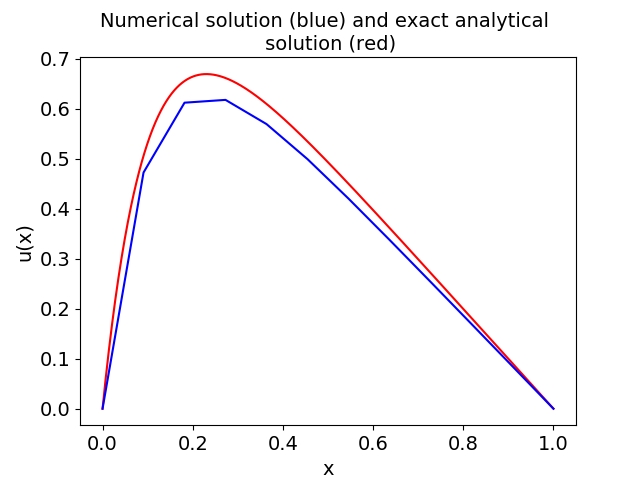
\includegraphics[width=10cm]{plot1b_10n.png}

\caption{n = 10 gridpoints.}
\label{fig:plott1}
\end{figure}

\begin{figure}[H]
\centering
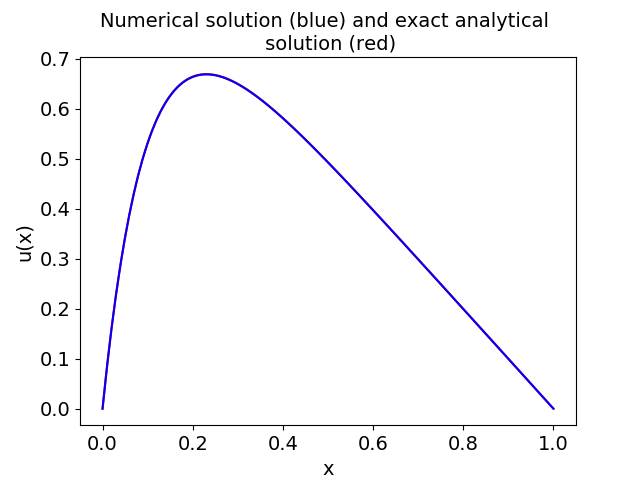
\includegraphics[width=10cm]{plot1b_100n.png}

\caption{n = 100 gridpoints. The numerical solution can't be separated visually 
from the exact solution.}
\label{fig:plott2}
\end{figure}

\begin{figure}[H]
\centering
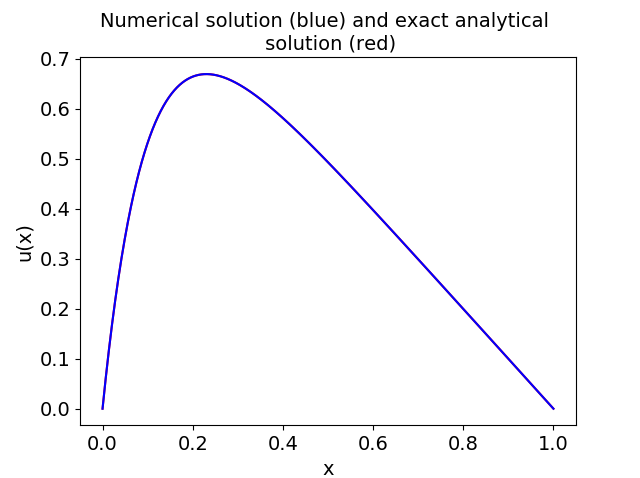
\includegraphics[width=10cm]{plot1b_1000n.png}

\caption{n = 1000 gridpoints. The numerical solution can't be separated visually 
from the exact solution.}
\label{fig:plott3}
\end{figure}

\noindent
Table (\ref{tabell1}) compares the time the computer's cpu spends on running through algorithm 1 with 
the time it spends on algorithm 2, for an increasing number
of grid points up to $n = 10^6$ points. The number of flops for each particular number of grid points
are also included in the table. Since algorithm 2  only need $4(n-1) + 1$ flops to find 
the discrete solution $\mathbf v$, which is just 50 percent compared to algorithm 1 's 
$8(n-1) + 1$ flops, we could actually
expect algorithm 2 to be twice as fast as algorithm 1. For the number of grid points used, 
both algorithm 1 and algorithm 2 are fast though. 
During the short time period the two algorithms are running, the cpu might
have other tasks to deal with too. This is one part of the reason why the difference in flops needed to 
run each of the
two algorithms isn't transfered to the difference in the time the cpu spends
on running them. The other part of the reason is that reading and writing to the computers internal
memory isn't taken into account. Anyway, table (\ref{tabell1}) shows that algorithm 2 always is faster than
algorithm 1 in our tests.

\vspace{4mm}
\noindent
Table (\ref{tabell2}) includes the cpu time spent in running through algorithm 3. 
The highest number of grid points are $n = 10^4$, and we clearly
see the pattern. Algorithm 3 is slower as expected, since it need in the order of 
$\frac{2}{3}n^3 + n^2$ flops to find the discrete solution $\mathbf v$. This is in the order of $n^2$ 
more flops than algorithm 1 needs to find $\mathbf v$. Again we have to consider that
reading and writing to the internal memory and other tasks the cpu might have affects the cpu times
measured.
Anyway, algorithm 3 is not an efficient algorithm to use when
we have a simple tridiagonal matrix $\mathbf A$.

\begin{table}[H]
\begin{center}
\begin{tabular}{|p{24mm}|p{52.25mm}|p{52mm}|}
\hline
 &\hspace{17mm}  cpu time    & \hspace{22mm} flops \\ \hline
\end{tabular}
\begin{tabular}{|p{24mm}|p{24mm}|p{24mm}|p{24mm}|p{24mm}|}
\hspace{8mm} n  & Algorithm1 & Algorithm2& Algorithm1& Algorithm2  \\ \hline 
\hspace{4mm} 10E+01 & 2.181E-05 & 2.021E-05  & 73 & 37  \\ \hline
\hspace{4mm} 10E+02 & 1.950E-04 & 1.293E-04  & 793& 397\\ \hline
\hspace{4mm} 10E+03 & 2.104E-03 & 1.382E-03& 7993&  3997\\ \hline
\hspace{4mm} 10E+04 & 2.068E-02 & 1.522E-02 & 79993& 39997 \\ \hline
\hspace{4mm} 10E+05 & 2.108E-01 & 1.627E-01& 799993& 399997\\ \hline
\hspace{4mm} 10E+06 & 2.097E+00 & 1.459E+00& 7999993& 3999997 \\ \hline
\end{tabular}
\end{center}
\caption{Comparison between algorithm 1 and algorithm 2: cpu time spent and number of
flops in the algorithms for n grid points (10E+1 means $10^1$).}
\label{tabell1}
\end{table} 


\begin{table}[H]
\begin{center}
\begin{tabular}{|p{25mm}|p{83.5mm}|}
\hline
 &\hspace{30 mm}  cpu time \\ \hline
\end{tabular}
\begin{tabular}{|p{25mm}|p{25mm}|p{25mm}|p{25mm}|}
\hspace{8mm} n  & Algorithm1 & Algorithm2& Algorithm3\\ \hline 
\hspace{4mm} 10E+01 & 2.182E-05 & 2.053E-05 & 2.665E-03   \\ \hline
\hspace{4mm} 10E+02 & 2.011E-04 & 1.347E-04 & 7.962E-04   \\ \hline
\hspace{4mm} 10E+03 & 2.116E-03 & 1.444E-03 & 4.597E-02   \\ \hline
\hspace{4mm} 10E+04 & 2.283E-02 & 1.587E-02 & 9.671E+00  \\ \hline
\end{tabular}
\end{center}
\caption{Comparison between the three algorithms: cpu time spent for n grid points.}
\label{tabell2}
\end{table} 

\noindent
Table (\ref{tabell3}) shows the maximum relative error in the discrete solution $v_i$ when it
is compared to the exact solution $u_i$ of expression (\ref{lig1}) in each grid point $i= 1, 2, \cdots, n$
for an increasing number of grid points up to $n=10^7$. 
The relative error is calculated as a function of $log_{10}$: 

\begin{equation*}
\epsilon_i = log_{10}\left(\Big\arrowvert\frac{v_i - u_i}{u_i}\Big\arrowvert\right)
\hspace{5mm} , i= 1, 2, \cdots, n
\end{equation*}
Figure(\ref{fig:plott4}) shows this relative error graphically.
The distance between each grid point is $h = 1/(n+1)$ and the term omitted in the basis for the
discrete approximation, see expression (\ref{lig2}), is of order $O(h^2)$. We therefore expect 
that when the number of gridpoints are multiplied by 10, the relative error will decrease with
a factor of $log_{10}(1/100) = -2$. The decrease in the relative error is as expected up to
$n = 10^5$. Between $n = 10^5$ and $n = 10^6$ the rate of relative error decrease is less steep
than $-2$, and for 
$n = 10^7$ the relative error has started to increase again. This is not due to the mathematical
approximations, but due to the limited number of bits the computer has
to represent a number. As $h$ becomes small, expression (\ref{lig2}), which form the basis
for the disctete approximation of $u(x)$, contains a subtaction between two nearly equal numbers:
$2u(x)-(u(x+h) + u(x-h))$. The resulting number of this subtraction will therefore not be represented
exactly in the computer. Its computer representation will loose significant bits. Loss of significant 
bits leads to round off errors in the numerical calculations,
and for $n = 10^7$ the accumulation of these errors have lead to a discrete
solution $\mathbf v$ with no better accuracy than for $n = 10^5$. 
See \cite{mhh} for a thorough explanation of computer 
representation of numbers and loss of significant bits.    


\begin{table}[H]
\begin{center}
\begin{tabular}{|p{25mm}|p{25mm}|}
\hline
\hspace{8mm} n  & \hspace{4mm} $\epsilon_i$\\ \hline 
\hspace{4mm} 10E+01 & -1.1797E+00 \\ \hline
\hspace{4mm} 10E+02 & -3.0880E+00 \\ \hline
\hspace{4mm} 10E+03 & -5.0801E+00 \\ \hline
\hspace{4mm} 10E+04 & -7.0793E+00 \\ \hline
\hspace{4mm} 10E+05 & -9.0776E+00 \\ \hline
\hspace{4mm} 10E+06 & -1.0122E+01\\ \hline
\hspace{4mm} 10E+07 & -9.0902E+00\\ \hline
\end{tabular}
\end{center}
\caption{Maximum relative error $\epsilon _i$ in the numerical solution 
$v_i,\hspace{3mm} i = 1, \cdots, n$.}
\label{tabell3}
\end{table} 

\begin{figure}[H]
\centering
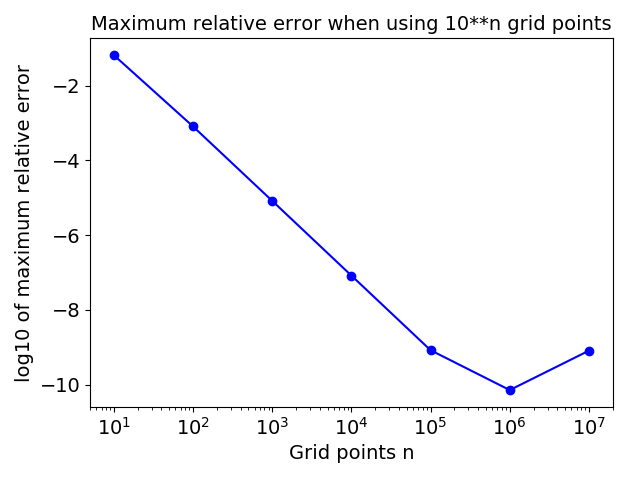
\includegraphics[width=10cm]{plot1d.png}

\caption{The maximum error $\epsilon_i$ from table (\ref{tabell3}).}
\label{fig:plott4}
\end{figure}

\vspace{4mm}
\noindent
Trying to use algorithm 3 together with $n=10000$ gridpoints result in the following error in
Python:

\begin{verbatim}
(base) M:\FYS4150-H19\Prosjekt1\Programmer>python Project1e_script.py
Traceback (most recent call last):
  File "Project1e_script.py", line 55, in <module>
    A = np.zeros((n,n))
MemoryError
\end{verbatim}

\noindent
Python simply don't accept a matrix $\mathbf{A}$ with $10^8$ floating point elements.
Too much of the computer's internal memory is used for just the matrix alone: 
$8\text{bytes}\times 10000^2 = 8\times 10^8\text{bytes}\approx 800 \text{Mbytes}$.
Since $\mathbf{A}$ is a tridiagonal matrix, a declaration of a $10000\times 10000$
matrix in order to use LU decomposition is just a waste of internal computer memory.


\subsection*{Conclusion}
We have programmed three different algorithms in the programming language Python
in order to find a numerical solution to the one-dimensional Poisson equation with
Dirichlet boundary conditions given in expression (\ref{lig1}). We have tested them
against a known analytical solution, and experienced that we can achieve an approximate
solution which converges toward the analytical solution as the number of gridpoints
n increases up towards $n = 10^7$. Then the loss of significant 
bits and acummulation of round off errors in the numerical calculations leads to
less accurate approximate solutions.

\vspace{5mm}
\noindent
The two algorithms, \emph{The general tridiagonal algorithm} and 
\emph{The special tridiagonal algorithm} are both efficient in solving the equation,
even though the \emph{The special tridiagonal algorithm} is somewhat faster since
it just contains half as many flops as \emph{The general tridiagonal algorithm}.
This could maybe lead us to believe that the computer's cpu would run through it 
twice as fast as \emph{The general tridiagonal algorithm}. According to our
time measurements, this is not the case, but in our tests 
\emph{The special tridiagonal algorithm} is always the fastest one.

\vspace{5mm}
\noindent
The \emph{The general LU decomposition algorithm} is the least efficient algorithm
of the three by a solid margin, since it need in the order of 
$n^2$ more flops to find the discrete solution $\mathbf v$ than 
\emph{The general tridiagonal algorithm}. Using LU decompsition in order to solve a 
matrix system $\mathbf{Av} = \mathbf{d}$ with a tridiagonal matrix 
$\mathbf A$ is time inefficient, and it also is uneccessary 
use of internal computer memory.


\newpage
\noindent
\begin{thebibliography}{9}
\bibitem[1]{mhh} Morten Hjort-Jensen: \emph{Course material in Computational Physics.}\\
http://compphysics.github.io/ComputationalPhysics/doc/web/course
\end{thebibliography}


\newpage
\noindent
\subsection*{Appendix: Computer programs}
The program language used is Python. In Python, the first index in vectors and matrices is $i = 0$,
not $i = 1$ which we used in the description of the algorithms in the Methods section. 
The indices in the programmed algorithms are therefore adjusted comparered to the presentation of
them in the Methods section, in order to be functional in Python. 
\emph{The general tridiagonal algorithm} and \emph{The special tridiagonal algorithm} are
programmed as two separate Python functions in a script called Diagonal\textunderscore Solvers.py
\emph{The general LU decomposition algorithm} is programmed as a function in a separate script
called LU\textunderscore Solver.py. 


\vspace{4mm}
\noindent
In the project description ,see \cite{mhh}, the programming tasks are separated into four
separate sub sections: Subsection 1b, 1c, 1d and 1e. These programming tasks are
separated into four separate Python scripts: Project1b\textunderscore script.py, 
Project1c\textunderscore script.py
Project1d\textunderscore script.py and Project1e\textunderscore script.py. 
These four scripts calls upon the three
algorithms when they are needed.

\vspace{4mm}
\noindent
Diagonal\textunderscore Solvers.py and LU\textunderscore Solver.py are included below.

\vspace{4mm}
\noindent
\textbf{Diagonal\textunderscore Solvers.py:}

\begin{verbatim}

import numpy as np
#import time
from time import perf_counter

def TriDiag(n,a,b,c,f):
    """
    Solves a system of n linear equations with n unknowns,
    when the matrix A in the nxn matrix system A*v = f is 
    tri-diagonal: 
    The array b of length n is the numbers on the diagonal of A. 
    If all the numbers are the same, b can be given as that single number.
    The array c of length n-1 is the numbers just above the diagonal of A. 
    If all the numbers are the same, c can be given as that single number.
    The array a of length n-1 is the numbers just below the diagonal of A. 
    If all the numbers are the same, a can be given as that single number.
    The rest of the numbers in A are equal to zero.
    """
    flop = 0
    #Checks out if b is a number. Assumes
    #then that the user has given a and c respectively as numbers too.
    if isinstance(b,(float,int)):
	    #Including an extra number in the array 'b' in order to make the array
        #compatible with the algorithm below.
        a = a*np.ones(n-1)
        b = b*np.ones(n)
        c = c*np.ones(n-1)
    else:
        #List 'a' converted to array 'a'. Also make
        #sure that array 'a' is a 'float' array, not an 'int' array.
        a = np.asarray(a)
        a = 1.0*a
        #a = np.hstack((0.0,a))
        #List 'b' converted to array 'b'. Also making sure that array 'b' is a
        #'float' array by multiplying it with 1.0.
        b = np.asarray(b)
        b = 1.0*b
  
        c = np.asarray(c)
        c = 1.0*c

    f = np.asarray(f)
    f = 1.0*f	
    v = np.zeros(n)

    #Starting timer
    start = perf_counter()
    #Forward substitution step:
    for i in range(1,n):
        d = (float(a[i-1])/b[i-1])
        b[i] = b[i] - d*c[i-1]
        f[i] = f[i] - d*f[i-1]
        flop = flop + 5

    #Backward substitution step
    v[n-1] =(f[n-1])/b[n-1]
    flop = flop + 1
    for i in range(n-1,0,-1):
        v[i-1] =(f[i-1] - c[i-1]*v[i])/b[i-1]
        flop = flop + 3
    #Elapsed cpu time while it is running the algorithm.
    slutt = perf_counter()
    total = slutt - start
    return v, flop, total




def TriDiagSpes(n,f):
    """
    Solves a system of n linear equations with n unknowns,
    when the matrix A in the nxn matrix system A*v = f is 
    tri-diagonal: 
    All the numbers of the diagonal of A is equal to 2.
    The numbers just above and below the diagonal is equal to -1.
    The rest of the numbers in A are equal to zero.
    """
    flop = 0
    a = -1*np.ones(n-1)
    b = 2*np.ones(n)
    c = -1*np.ones(n-1)
   
    #List 'f' converted to array 'f'. Also making sure that array 'f' is a
    #'float' array by multiplying it with 1.0.
    f = np.asarray(f)
    f = 1.0*f	
	
    v = np.zeros(n)

    #Starting timer
    start = perf_counter()
    #c0 = time.time()
    #Forward substitution step:
    for i in range(1,n):
        b[i] = float((i+2))/(i+1)
        f[i] = f[i] + ((float(i))/(i+1))*f[i-1]
        flop = flop + 2

    #Backward substitution step
    v[n-1] = (f[n-1])/b[n-1]
    flop = flop + 1
    for i in range(n-1,0,-1):
        v[i-1] = (float(i)/(i+1))*(f[i-1] + v[i])
        flop = flop + 2
    #Elapsed cpu time while it is running the algorithm.
    slutt = perf_counter()
    total = slutt - start
    return v,flop,total




#Testing of the two tridiagonal solvers
"""
a = -1
b = 2
c = -1
n = 4
f = [1,2,3,4]

print('--------------------------')
print('Testing of the general tridiagonal solver:')
[v1,flop_g, total_g] = TriDiag(n,a,b,c,f)
print('v = %s'%v1)
print('Floating Point Operations for n = %d: %d'%(n,flop_g))
print('Elapsed CPU time: %G s'%total_g)


print('--------------------------')
print('Testing of the special tridiagonal solver:')
[v2,flop_s, total_s] = TriDiagSpes(n,f)
print('v = %s'%v2)
print('Floating Point Operations for n = %d: %d'%(n,flop_s))
print('Elapsed CPU time: %G s'%total_s)
"""

#The result of the testing
"""
(base) M:\FYS4150-H19\Prosjekt1\Programmer>python Diagonal_Solvers.py
--------------------------
Testing of the general tridiagonal solver:
v = [4. 7. 8. 6.]
Floating Point Operations for n = 4: 25
Elapsed CPU time: 1.7965E-05 s
--------------------------
Testing of the special tridiagonal solver:
v = [4. 7. 8. 6.]
Floating Point Operations for n = 4: 13
Elapsed CPU time: 1.7002E-05 s
"""


\end{verbatim}

\vspace{4mm}
\noindent
\textbf{LU\textunderscore Solver.py}

\begin{verbatim}

import numpy as np
import scipy.linalg as scl
from time import perf_counter


def LU_Solver(A,f,n):
    """
    Solves a system of n linear equations with n unknowns with
    the aid of LU decomposition of the matrix A : A*v = f => (L*U)*v = f
    => U*v = (inverse(L))*f. Then y = inverse(L)*f and we find v with
    backward substitution of y = U*v   
    """
    y = np.zeros(n)
    v = np.zeros(n)

    #Starting timer
    start = perf_counter()

    #LU decomposition of quadratic matrix A
    P,L,U = scl.lu(A)

    #Inverting L
    #LL = scl.inv(L)
    #Matrix multiplication between matrix LL and vector f
    #y = np.dot(LL,f)
	
    #Forward substitution to find vector y = L**(-1)*f
    for i in range(n):
        y[i] = f[i] - np.dot(L[i,:],y) 	

    #Backward substitution to find solution vector v
    for i in range(n-1,-1,-1):
        v[i] = (float(y[i] - np.dot(U[i,:],v)))/U[i,i]

    #Elapsed cpu time during the run of the algoritm.
    slutt = perf_counter()
    total = slutt - start
    return v, total


#Testing of the LU solver
"""
a = -1
b = 2
c = -1
f = np.asarray([1,2,3,4])
f = 1.0*f

n = 4
A = np.zeros((n,n))
A[0,0] = b
A[0,1] = c
A[n-1,n-1] = b
A[n-1,n-2] = a

for i in range(1,n-1):
    A[i,i] = b
    A[i, i -1] = a
    A[i,i+1] = c

print('Testing of the LU solver:')
[v,Total_LU] = LU_Solver(A,f,n)
print('v = %s'%v)
print('Elapsed CPU time: %G s'%Total_LU)
"""

#The result of the testing
"""
(base) M:\FYS4150-H19\Prosjekt1\Programmer>python LU_Solver.py
Testing of the LU solver:
v = [4. 7. 8. 6.]
Elapsed CPU time: 0.00305115 s
"""

\end{verbatim}


\end{document}











%\paragraph{Outline}
%First we start with a little example of the article class, which is an 
%important documentclass. But there would be other documentclasses like 
%book \ref{book}, report \ref{report} and letter \ref{letter} which are 
%described in Section \ref{documentclasses}. Finally, Section 
%\ref{conclusions} gives the conclusions.



%\section{Documentclasses} \label{documentclasses}

%\begin{itemize}
%\item article
%\item book 
%\item report 
%\item letter 
%\end{itemize}


%\begin{enumerate}
%\item article
%\item book 
%\item report 
%\item letter 
%\end{enumerate}

%\begin{description}
%\item[article\label{article}]{Article is \ldots}
%\item[book\label{book}]{The book class \ldots}
%\item[report\label{report}]{Report gives you \ldots}
%\item[letter\label{letter}]{If you want to write a letter.}
%\end{description}


%\section{Conclusions}\label{conclusions}
%There is no longer \LaTeX{} example which was written by \cite{doe}.





